
%%%%%%%%%%%%%  Start of GENERATED TEXT  %%%%%%%%%%%%\n

\newpage
\setcounter{page}{5}
\setcounter{section}{0}
\setcounter{equation}{0}
\setcounter{figure}{0}
\setcounter{table}{0}
\setcounter{footnote}{0}
\renewcommand{\figurename}{Fig.}
\renewcommand{\ehkol}{Author1 N. S., Author2 N. S.}
\renewcommand{\ohkol}{Title of Paper in English\ldots}
\Vykh{radap1xxx:FirstPage}{radap1xxx:LastPage}
\begin{multicols}{2}
[
\UDC{621.39} %\noUDC{}
\renewcommand{\ehkol}{Автор1 І. Б., Автор2 І. Б.}
\renewcommand{\ohkol}{Назва статті \ldots}
\Title{Шаблон оформлення статті для журналу <<Вісник НТУУ ``КПІ''. Серія Радіотехніка. Радіоапаратобудування>>}\label{radap1ххх:FirstPage}
\Authors{Автор1 І. Б., Автор2 І. Б.}
\aff{Харківський національний університет радіоелектроніки, м. Харків, Україна\\Національний університет ``Львівська політехніка'', м. Львів, Україна}
\Address{}{\href{mailto:author@email.ua}{authorv@email.ua}}
\AbsKeywords{У роботі представлені вимоги щодо оформлення статей для подання у збірник наукових праць ``Вісник Національного технічного університету України <<Київський політехнічний інститут>>. Серія Радіотехніка. Радіоапаратобудування''. Показано, що дотримання встановлених правил дозволить покращити вашу статтю .
}
{Ключові слова}{правила оформлення, радіотехніка, радіоапаратобудування, \LaTeX}
{\href{http://radap.kpi.ua/radiotechnique/article/view/1xxx}{10.20535/RADAP.2023.93.\pageref{radap1ххх:FirstPage}-\pageref{radap1ххх:LastPage}}}
]

%
%

\pdfbookmark[1]{Вступ}{intro}
\section*{Вступ}
Шановні автори, даний документ є прикладом оформлення статті в редакторі \LaTeX\ для публікації у журналі <<Вісник Національного технічного університету України ``Київський політехнічний інститут''. Серія Радіотехніка. Радіоапаратобудування>>. У разі використання запропонованого редакцією шаблону всі правила оформлення будуть застосовані автоматично.

\section{Порядок проходження рукописів статей}
Усі рукописи статей слід подавати через форму на сайті. Для цього необхідно зареєструватися на сайті та пройти 5 кроків слідуючи детальним інструкціям. У разі якщо у статті оформлені метадані трьома мовами (назва, анотація, ключові слова, прізвища авторів у транслітерації) процес подання займе не більше 5-ти хвилин. Формат документів, у якому подається рукопис на рецензування може бути: \texttt{*.pdf}, \texttt{*.tex}, \texttt{*.doc}. Розмір не повинен перевищувати 4 МБ. Проте у разі успішного проходження рецензування рукопис слід оформити у редакторі \LaTeX\ з використанням запропонованого редакцією стильового файлу.

Проходження статей до друку відбувається у декілька етапів:
\begin{list}{-}{}
	\item реєстрація подання через сайт \texttt{radap.kpi.ua};
	\item рецензування (до 2-х місяців);
	\item літературна корекція;
	\item редакторська підготовка;
	\item публікація випуску.
\end{list}  

Періодичніть друку 4-ри рази на рік: 
\begin{enumerate}
	\begin{multicols}{2}
	\item 30 березня, 
	\item 30 червня, 
	\item 30 вересня, 
	\item 30 грудня.
	\end{multicols}
\end{enumerate}

\section{Вимоги до оформлення}

Статті повинні мати такі необхідні елементи: 
\begin{list}{-}{}
	\item постановка задачі; 
	\item аналіз досліджень і публікацій, в яких започатковано розв'язання даної задачі; 
	\item виділення невирішених частин загальної проблеми, котрим присвячується означена стаття; 
	\item формулювання цілей статті; 
	\item виклад матеріалу дослідження; 
	\item обговорення (аналіз) приведених у статті результатів, порівняння з результатами інших дослідників; 
	\item висновки з даного дослідження, перспективи його подальшого розвитку.
\end{list}

У зв'язку з цим науково-технічні статті та повідомлення про досягнення науково-практичних результатів мають бути структурованими - поділеними на розділи з заголовками. Наприклад, для науково-технічних статей: вступ, постановка задачі, теоретичні викладки, методика та засоби експериментальних досліджень, принципи побудови та схемно-конструкторські особливості розробленої апаратури, результати експериментів та випробувань розробленої апаратури, обговорення та оцінка отриманих результатів з вже відомими, висновки та рекомендації.

Статті можуть бути опубліковані однією  з двох мов --- українською,  англійською. Метадані (Назва, анотація, ключові слова) надаються двома мовами (українською та англійською). Обсяг анотації 10 - 12 рядків. Англійська анотація має бути розширеною та структурованою відповідно до структури статті з відображенням основних отриманих результатів.

Обсяг рукопису має становити 5 -- 7 повних сторінок формату А4 (включаючи рисунки, таблиці, перелік посилань, анотації та ключові слова).

У рукописах слід дотримуватись термінології, прийнятої державними стандартами; у разі використання нових термінів або абревіатур, слід їх розшифрувати та пояснити у тексті.



\section{Приклади оформлення окремих елементів статті}


\subsection{Формули}
Формули можуть розміщуватися у тексті: $\mathbf{\eta}_0$, $E\left\lbrace \hat{\mathbf{\eta}}\right\rbrace = \mathbf{\eta}_0$ або їх можна виокремити окремим рядком.  Для того, щоб можливо було оформити посилання на формулу, слід використовувати мітки, наприклад: \texttt{$\backslash$label\{eq1\}}. Далі зробити посилання на це рівняння можна за допомогою виразу: \texttt{$\backslash$eqref\{eq1\}}. Таким чином можливо здійснити автоматичну нумерацію формул.

\begin{equation}\label{eq1}
H(A)=-\sum \limits_{i=1}^n p_i \log p(p_i)
\end{equation}


Декілька рівнянь з позначкою одним номером:
\begin{equation}
\begin{aligned}\label{eq2}
\rho_{+mn}^E &=\frac{Z_0-Z_{B_{mn}}^E}{Z_0-Z_{mn}^E} =-\rho_{+mn}^H \\
\rho_{+mn}^H &=\frac{\sqrt{1-\left( \frac{m\lambda}{2b_p}\right) ^2-\left( \frac{m\lambda}{2a_p}\right) ^2}-1 }{\sqrt{1-\left( \frac{m\lambda}{2b_p}\right) ^2-\left( \frac{m\lambda}{2a_p}\right) ^2}+1}
\end{aligned}
\end{equation}

Довгі формули слід записувати у декілька стрічок як це приведено нижче:
\begin{multline}\label{radap1345eq2}
U_{i-1}= \sum\limits_{j=0}^{i-1}\left| r_j - \sum\limits_{h=0}^{g} x_{(j-h)} \nu_h \right|^2 =\\= \sum\limits_{j=0}^{i-2}\left| r_j - \sum\limits_{h=0}^{g} x_{(j-h)} \nu_h \right|^2 +w_{i-1} =\\= U_{i-2} + w_{i-1} 
\end{multline}

Дуже довгі формули, що варко розмістити в одній колонці можна розмістити на всю сторінку як це приведено нижче:

\end{multicols} % Закриваємо розмітку на дві колонки

\begin{align}\label{radap1333eq17} % Формула на всю сторінку
\begin{split}
A_{+m_x m_y}^{H_\perp} \cong -4E_0a_pe^{-inkd_y\sin\theta_\text{П}}\frac{a_p(1+\cos \theta_\text{П})}{(m_y\pi)^2} 
\frac{\sin^2{(\frac{m_y\pi}{2})}\cos{(\frac{ka_p}{2}\sin{\theta_\text{П}})}+i\cos^2{(\frac{m_y\pi}{2})}\sin{(\frac{ka_p}{2}\sin{\theta_\text{П}})}}{\left( 1+\sqrt{1-\left( \frac{m_y\lambda}{2a_p}\right) ^2}\right) \left( 1-\rho_{-mn}^H \rho_{+mn}^H \left( 1-\left( \frac{2a_p}{m_y\lambda}\sin\theta_\text{П}\right) ^2\right) \right)  }
\end{split}	 
\end{align}	

\begin{multicols}{2} % Відкриваємо нову розмітку на дві колонки


\subsection{Рисунки}
Всі рисунки в статті бажано оформляти у векторному вигляді і зберігати їх в форматі \texttt{.pdf}. Оформити векторні рисунки можливо у програмах \textit{Visio}, \textit{Corel~Draw}, \textit{Microsoft Office}, \textit{TikZ} та ін. Також можливо вставляти растрові малюнки у форматі \texttt{*.png} або \texttt{*.jpeg} з якістю, що є достатньою для якісного друку (не менше \texttt{300dpi}). Файли рисунків мають бути розміщені в одній директорії з текстовим файлом. Маштабування задається як параметр до команди вставки рисунку. Приклади вставки рисунків приведено на рис. \ref{fig1} та \ref{fig2}. Мітки для рисунків оформляються агналогічно формулам, автоматичні посилання на рbсунок можливо здійснити командою \texttt{$\backslash$ref\{label\}}.


\begin{Figure}\centering%{l}{\linewidth}
	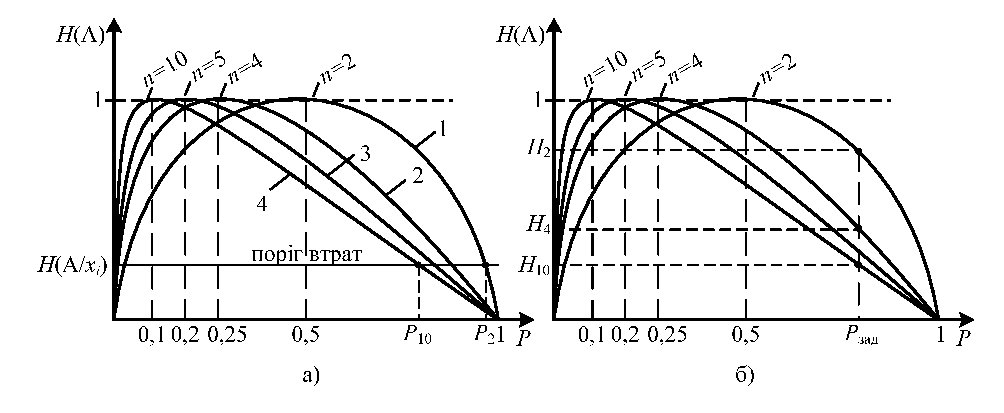
\includegraphics[width=\linewidth]{fig1}
	\captionof{figure}{Підпис до рисунку}\label{fig1}
\end{Figure}

\begin{figure*}\centering
	%Figure 5 	
	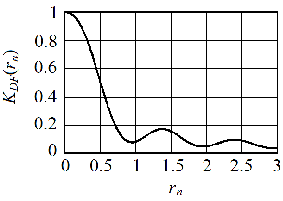
\includegraphics[width=0.4\linewidth]{fig2a}
	~~~~~
	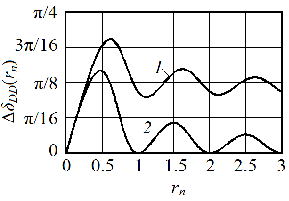
\includegraphics[width=0.4\linewidth]{fig2b}
	\begin{tabular}{p{0.49\linewidth}p{0.49\linewidth}}
		\centering (a) & \centering (b)  
	\end{tabular}	
	\captionof{figure}{Підпис до рисунку (a) $\Delta\delta_{DD}(r_n)$ (b)  $\theta = 1 $}\label{fig2}%
\end{figure*}



\subsection{Таблиці}

Таблиці можуть мати заголовок, розміщений над таблицею. 
\begin{Table}
	\captionof{table}{Заголовок таблиці}
	\begin{tabularx}{\linewidth}{|l|X|c|}
		\hline 
		\multirow{2}{4em}{\rule{0pt}{11pt} Param} & \multicolumn{2}{c|}{\rule{0pt}{11pt} Models}\\ 
		\cline{2-3} 
		             & $K$ &  $S$\\ 
		\hline 
		\rule{0pt}{10pt}$p=0,001$& $1,2359\times V^{0,1241}-1,3399$ &  0,00158\\ 
		\hline 
		\rule{0pt}{10pt}$p=0,005$& $-8,3753\times V^{-0,0274}+8,2477$ &  0,00150\\ 
		\hline 
		\rule{0pt}{10pt}$p=0,01$&  $2,7669\times V^{-0,0983}+2,6440$&  0,00092\\ 
		\hline 
		\rule{0pt}{10pt}$p=0,02$&  $-1,8264\times V^{-0,1769}+1,7115$&  0,00072\\ 
		\hline 
		\rule{0pt}{10pt}$p=0,05$&  $-1,3804\times V^{-0,2872}+1,3013$&  0,00045\\ 
		\hline 
		\rule{0pt}{10pt}$p=0,001$&  $1,6368\times Z^{0,736}-1,4640$&  0,00023\\ 
		\hline 
		\rule{0pt}{10pt}$p=0,005$&  $3,1652\times Z^{0,0420}-2,9549$&  0,00041\\ 
		\hline 
		\rule{0pt}{10pt}$p=0,01$&  $-6,2994\times Z^{-0,0244}+6,5212$&  0,00031\\ 
		\hline 
		\rule{0pt}{10pt}$p=0,03$&  $-2,2772\times Z^{-0,0749}+2,5429$&  0,00012\\ 
		\hline 
	\end{tabularx} \label{radap1361tab1}
\end{Table}

\section{Оформлення посилань}

Перелік посилань подається в порядку згадування у тексті та має бути оформлений згідно ДСТУ-ГОСТ 7.1:2006 та у транслітерації стилем Harvard. У разі якщо всі джерела є англомовними посилання слід оформляти без транслітерації, але з використанням стилю Harvard.

Приклад оформлення посилань  \cite{ref1,ref4} за допомогою команди \texttt{$\backslash$cite\{label1, label4\}}. 



\pdfbookmark[1]{Висновки}{conc}
\section*{Висновки}
Рукопис оформлений відповідно до цього шаблону слід надсилати у редакцію через офіційний сайт, після чого до Вас на електронну пошту прийде підтвердження отримання рукопису. Далі редактор виконає формальну перевірку рукопису на відповідність вимогам до оформлення статей та направить його на рецензування. Матеріали, що оформлені з відхиленнями від встановлених вимог можуть направляютися авторам на доопрацювання. У разі виникнення запитань звертайтесь до редакції за тел. \texttt{+380 44 204 93 29} або електронною поштою \texttt{radap@rtf.kpi.ua}.



\pdfbookmark[1]{Перелік посилань}{lit}
\section*{Перелік посилань}
\begin{enumerate}\footnotesize
	\item Войтер А.П.  Комплексний аналіз ефективної швидкості передачі в адаптивних пакетних радіомережах~/ А.П.~Войтер  // Наукові вісті НТУУ ``КПІ''.~-- 2013.~-- № 6.~-- с. 7-12.
	\item Razeghi M. The Wonder of Nanotechnology: Quantum Optoelectronic Devices and Applications / M. Razeghi, L. Esaki, K. von Klitzing, eds.~--  Bellingham: SPIE Press.~--  2013.~--  1000\,p.
	\item Massaro A. Photonic Crystals~--  Introduction, Applications and Theory / A. Massaro, ed.~--  Publisher: InTech.~--  2012.~--  356\,p.
	\item Khelif A., Adibi A. Phononic Crystals: Fundamentals and Applications / Khelif A., Adibi A., eds.~--  N. Y.: Springer.~--  2015.~--  268\,р.
	\item Brillouin L. Wave Propagation in Periodic Structures: Electric Filters and Crystal Lattices / L. Brillouin.~--  N.~Y.\,: McGraw–Hill.~--  1946 (1st ed.); Dover.~--  1953 (2nd ed. corrections and additions); Courier Corporation (unabridged republication of 2nd ed.).~--  2003.~--  260 p.
	\item Бриллюэн Л. Волны в перидических структурах / Л. Бриллюэн, М. Пароди.~--  М. : Изд. иностр. лит.~--  1956.~--  457\,с.
	\item Markos P. Wave Propagation From Electrons to Photonic Crystals and Left-Handed Materials / P. Markos, C. M. Soukoulis.~--  Princeton and Oxford: Princeton University Press.~--  2008.~--  352\,p.
	\item Нелин Е. А. Моделирование и повышение избирательности кристаллоподобных структур / Е. А. Нелин // ЖТФ.~--  2004.~--  Т. 74, № 11.~--  С. 70-74.
	\item Нелин Е. А. Краевая аподизация кристаллоподобных структур / Е. А. Нелин // ЖТФ.~-- 2005.~-- Т. 75, № 11.~-- С. 120-121.
	\item Водолазская М. В. Модель импедансных дельта-неоднородностей для микро- и наноструктур / М. В. Водолазская, Е. А. Нелин // Известия вузов. Радиоэлектроника.~-- 2014.~-- Т. 57, № 5.~-- С. 25-34.
\end{enumerate}

\pdfbookmark[1]{References}{translit}
\renewcommand{\refname}{References}

\begin{thebibliography}{99}\footnotesize
	
	\bibitem{ref1} Voiter A.P. (2013) Comprehensive Analysis of the Effective Rate in Adaptive Packet Radio Networks. \href{http://old.bulletin.kpi.ua/en/taxonomy/term/3023}{\textit{Naukovi visti NTUU ``KPI''}}, No 6, pp. 7-12.
	
	\bibitem{ref2} Razeghi M., Esaki L. and Klitzing K. (2013) \href{http://dx.doi.org/10.1117/3.1002245}{\textit{The Wonder of Nanotechnology: Quantum Optoelectronic Devices and Applications}}, Bellingham, SPIE Press, 1000 p. DOI: 10.1117/3.1002245
	
	\bibitem{ref3} Massaro A. (2012) \href{http://dx.doi.org/10.5772/1971}{\textit{Photonic Crystals – Introduction, Applications and Theory}}, InTech Publisher, 356 p. DOI: 10.5772/1971
	
	\bibitem{ref4} Khelif A. and Adibi A. (2015) \href{http://dx.doi.org/10.1007/978-1-4614-9393-8}{\textit{Phononic Crystals: Fundamentals and Applications}}, N. Y., Springer, 268 p. DOI: 10.1007/978-1-4614-9393-8
	
	\bibitem{ref5} Brillouin L. (2003) \href{https://books.google.com.ua/books?id=m2WmGiU5nUwC}{\textit{Wave Propagation in Periodic Structures: Electric Filters and Crystal Lattices, 2nd ed}}, Dover Publications, 260 p.
	
	\bibitem{ref6} Brillouin L. and Parodi M. (1956) \href{https://books.google.com.ua/books?id=ltPQAAAAMAAJ}{\textit{Propagation des ondes dans les milieux p{\'e}rodiques}}. Paris, Masson et Cie, 347 p.
	
	\bibitem{ref7} Markos P. and Soukoulis C. M. (2008) \href{http://dx.doi.org/10.1515/9781400835676}{\textit{Wave Propagation From Electrons to Photonic Crystals and Left-Handed Materials}}. Princeton and Oxford: Princeton University Press, 352 p. DOI: 10.1515/9781400835676
	
	\bibitem{ref8} Nelin E. A. (2004) Simulation and improvement of the selectivity of crystal-like structures. \href{http://dx.doi.org/10.1134/1.1826191}{\textit{Tech. Phys.}}, Vol. 49, No. 11, pp. 1464-1468. DOI: 10.1134/1.1826191
	
	\bibitem{ref9} Nelin E. A. (2005) Edge apodization of crystal-like structures. \href{http://dx.doi.org/10.1134/1.2131963}{\textit{Tech. Phys.}}, vol. 50, no. 11, pp. 1511-1512. DOI: 10.1134/1.2131963
	
	\bibitem{ref10} Vodolazka M. V. and Nelin E. A. (2014) Model of impedance delta-inhomogeneities for micro- and nanostructures. \href{http://dx.doi.org/10.3103/s0735272714050033}{\textit{Radioelectronics and Communications Systems}}, Vol. 57, No. 5. pp. 208-216. DOI: 10.3103/s0735272714050033
	
\end{thebibliography}  

\TitleSecond{Title of Paper in English}

\Auth{Author1 N. S., Author2 N. S.}

\AbsK{The article estimates the value of informative monitoring features and signatures their efficiency as a measure of ambiguity during recognition sources and objects for monitoring in the information environment of telecommunication systems which are appropriate to assess by magnitude of loss of information. The main idea of the research. The process and mechanism of evaluating information while losses signatures formed on the basis of the monitoring features are considered. Conclusion. Formed appropriate signatures are used in the process of recognition and have basis for decision which of sources belonging to class or operative (phase) state facilities. Optimum numbers of monitoring features in recognition sources object monitoring and optimal number of signatures for identify a source or object are defined.}
{Key words}
{monitoring features; signatures; informational losses; entropy}

\label{radap1ххх:LastPage}
\end{multicols}
\newpage
%%%%%%%%%%%%%  END of GENERATED TEXT  %%%%%%%%%%%%\n

